\section{Durchführung}
\label{sec:Durchführung}
Der Versuchsaufbau besteht aus einem Schwingungsgenerator mit
integriertem Tiefpass, sowie einem gewöhnlichen Oszilloskop.
\subsection{Entladekurve eines Kondesators}
Es soll die Zeitkonstante $RC$ bestimmt werden. Dazu wird das in 
\autoref{fig:Schalung_Entladung} gezeigte Schaltbild verwendet.
\begin{figure}
    \centering
    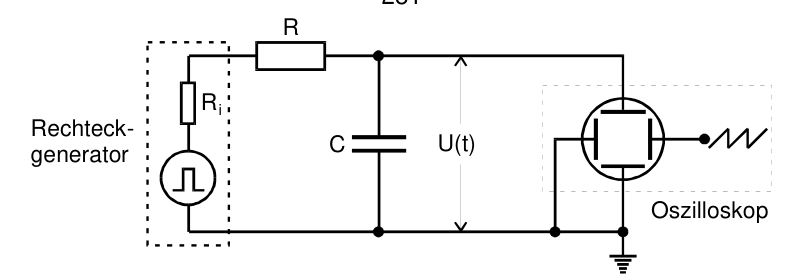
\includegraphics[width=\textwidth]{messdaten/Schaltung_Entladung.png}
    \caption{Das zur Bestimmung der Zeitkonstante $RC$ verwendete Schaltbild.}
    \label{fig:Schalung_Entladung}
\end{figure}
Der Wellengenerator gibt für diesen Teilversuch eine Rechtecksspannung aus.
Auf dem Oszilloskop wird dann eine Entladekurve der Spannung in Abhängigkeit
der Zeit dargestellt, welche in \autoref{fig:Entladekurve} skizziert ist.
\begin{figure}
    \centering
    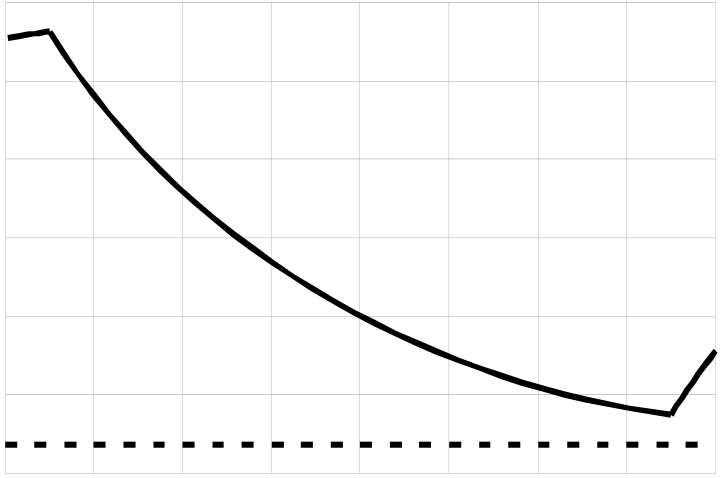
\includegraphics[height=4.5cm]{messdaten/Entladekurve.png}
    \caption{Skizze einer Entladekurve des Kondensators. Auf der y-Achse ist
    die Spannung $U$ aufgetragen, auf der x-Achse die Zeit $t$. Die gestrichelte
    Linie stellt $U(t)=0$ dar.}
    \label{fig:Entladekurve}
\end{figure}
Bei einer Frequenz von $\qty{200}{\hertz}$ werden 15 Punkte der Kurve aufgenommen. 
\subsection{Bestimmung der Frequenzabhängigkeit von Phasenverschiebung und Amplitude}
Es werde bei gleichem Versuchsaufbau zwei Sinuswellen generiert.
Die Eine dient als Referenz und bildet die Erregerspannung ab.
Die zweite Welle zeigt die Kondensatorspannung.
In einem Frequenzbereich von $\qty{5}{\hertz}$ bis $\qty{6}{\kilo\hertz}$ werden jeweils
die Amplitude der Kondensatorspannung, die Phasenverschiebung sowie die Periodenlänge
gemessen.
\subsection{Integration der Spannungsfunktion}
Mittels des Schaltbildes in \autoref{fig:Schaltung_b_c} und drei verschiedenen
Schwingungsformen soll gezeigt werden, dass diese Schaltung auch als Integrator fungieren 
kann. Die drei Schwingungsformen sind Sinus-, Dreiecks-, sowie Rechteckförmige Schwingungen.
Dabei muss die angelegte Frequenz größer als $\sfrac{1}{RC}$ sein. Dann werden die vertikalen 
Positionen beider Kurven jeweils so angepasst, dass beide zu sehen sind. Von jeder Schwingung 
sowie der Stammfunktion wird ein Foto gemacht.
\begin{figure}
    \centering
    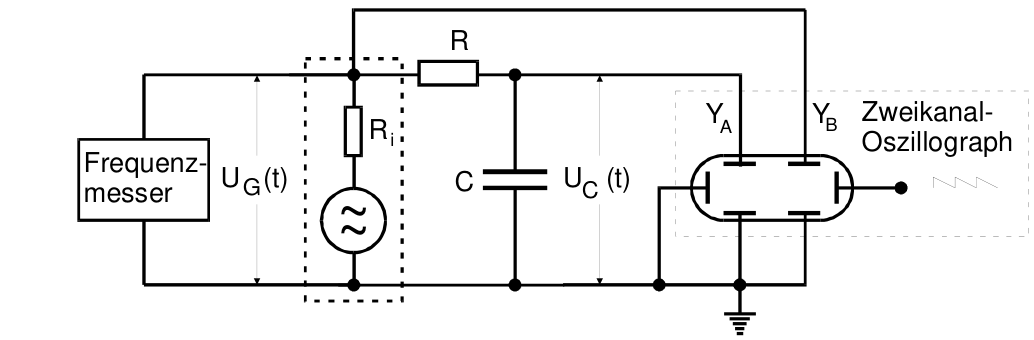
\includegraphics[height=5cm]{messdaten/Schaltung_b_c.png}
    \caption{Die für Teilaufgabe b) und c) verwendete Schaltung.}
    \label{fig:Schaltung_b_c}
\end{figure}